\begin{activite}[Ordre des opérations]

\begin{partie}[Le mauvais ordre]
Voici le calcul qui a été proposé aux 23 élèves d’une classe de 8e : $3 + 6 \times 7$. Voici les résultats obtenus : \\[0.5em]
\begin{center}
\begin{tabularx}{.8\linewidth}{|c|*{6}{>{\centering \arraybackslash}X|}}
\hline \rowcolor{G3} Résultat & 45 & 63 & Autres \\
\hline \rowcolor{F3} Nombre d'élèves & 11 & 10 & 2 \\
\hline
\end{tabularx}
\end{center}

\begin{enumerate}
 \item Explique comment les élèves ont trouvé les résultats 45 et 63 ;
 \item En observant les quatre calculs ci-dessous, qui sont corrects, énonce la règle de priorité :
          \begin{colitemize}{2}
           \item $15 - 2 \times 3 = 9$ ;
          \item $7 \times 8 + 10 = 66$ ;
          \item $27 + 35 \div 5 = 34$ ;
           \item $60 - 12 \div 4 = 57$ ;
           \end{colitemize} 
 \item Calcule $9 - 9 \times 0,5$ puis $9 \times 7 - 8 \div 4$.   
 \end{enumerate}

\end{partie}

\begin{partie}[Lire dans le bon sens]
\begin{enumerate}
 \item Calcule $K = 4 + 12 - 3 + 7$ \dotfill

\dotfill

 \item Un professeur a programmé deux feuilles, sur un tableur, pour montrer les étapes de calcul. En observant les captures d'écran ci-dessous, énonce la règle : \\[1em]
 \begin{minipage}{0.4\textwidth}
  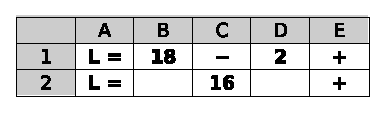
\includegraphics[width=5.5cm]{tableau1}
  \end{minipage} \hfill%
   \begin{minipage}{0.4\textwidth}
    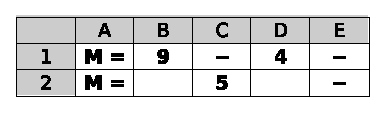
\includegraphics[width=5.5cm]{tableau2}
    \end{minipage}\\
 \item Calcule, en écrivant les étapes :  

$N = 21 - 9 - 3$ \dotfill

$P = 17 - 8 + 1$ \dotfill

 \item Dans l'expression $K$, où dois-tu placer des parenthèses pour obtenir 6 comme résultat ?

\dotfill
 \end{enumerate}
\end{partie}

\end{activite}

%%%%%%%%%%%%%%%%%%%%%%%%%%%%%%%%%%%%%%%%%%%%%%%%%%%%%%%%%%%

\begin{activite}[Les deux calculatrices]

 \begin{minipage}{0.6\textwidth}
Hervé et Bruno ont tous deux acheté une calculatrice. Hervé a choisi une calculatrice performante avec laquelle il peut écrire les formules. Bruno, lui, a acheté une petite calculatrice solaire. Ils cherchent à calculer $4 + 3 \cdot 8$.

Tous les deux appuient successivement sur les touches suivantes :  \\[0.5em]
\begin{tabular}{|c|c|c|c|c|c|c|c|c|c|c|}
\cline{1-1} \cline{3-3}\cline{5-5} \cline{7-7}\cline{9-9} \cline{11-11}
4 & & + & & 3 & & $\times$ & & 8 & & = \\ \cline{1-1} \cline{3-3}\cline{5-5} \cline{7-7}\cline{9-9} \cline{11-11}
\end{tabular} \\[0.5em]
Hervé obtient 28 comme résultat et Bruno obtient 56.
 \end{minipage} \hfill%
  \begin{minipage}{0.2\textwidth}
   
\includegraphics[width=3.5cm]{calculette}
   \end{minipage}\\

\begin{partie}
Qui a le bon résultat ?
\end{partie}

\begin{partie}
Les deux calculatrices fonctionnent très bien. Comment expliques-tu ces résultats différents ?
\end{partie}

\begin{partie}
Après réflexion, Bruno a trouvé une méthode pour obtenir le bon résultat avec sa calculatrice solaire. Quelle est cette méthode ?
\end{partie}

\end{activite}

%%%%%%%%%%%%%%%%%%%%%%%%%%%%%%%%%%%%%%%%%%%%%%%%%%%%%%%%%%%

\begin{activite}[Attention à la présentation]

 \begin{partie}
Mélanie et Aïssatou ont effectué le même calcul dont voici le détail ci-dessous. L'une d'entre elles s'est trompée. Indique laquelle et explique son erreur :

\vspace{1em}

\begin{center}
 \begin{tabularx}{.6\linewidth}{X|cX}
  \multicolumn{1}{c|}{Mélanie} & \multicolumn{2}{c}{Aïssatou} \\
  $A = \underline{8 \cdot 4} - 7 \cdot 3$ && $A = \underline{8 \cdot 4} - 7 \cdot 3$ \\
  $A = \underline{32 - 7} \cdot 3$ && $A = 32 - \underline{7 \cdot 3}$ \\
  $A = \underline{25 \cdot 3}$ && $A = \underline{32 - 21}$ \\
  $A = 75$ && $A = 11$ \\
  \end{tabularx}
\end{center}

\end{partie}


\begin{partie}
Mélanie et Aïssatou ont un second calcul à effectuer dont voici le détail ci-dessous. Aïssatou n'a pas réussi à terminer son calcul. Indique son erreur :

\vspace{1em}

\begin{center}
 \begin{tabularx}{.6\linewidth}{X|cX}
  \multicolumn{1}{c|}{Mélanie} & \multicolumn{2}{c}{Aïssatou} \\
  $A = 18 - \underline{(2 + 3)}$ && $A = 18 - \underline{(2 + 3)}$ \\
  $A = \underline{18 - 5}$ && $A = \underline{5 - 18}$ \\
  $A = 13$ && $A = ??$ \\
  \end{tabularx}
\end{center}

\end{partie}

\end{activite}


%%%%%%%%%%%%%%%%%%%%%%%%%%%%%%%%%%%%%%%%%%%%%%%%%%%%%%%%%%%

\begin{activite}[Avec des barres]

\textbf{Notation :}

L’écriture $\dfrac{10}{(2 + 3)}$ correspond à $10 / (2 + 3)$ ou encore à $10 : (2 + 3)$.

Autrement dit : $\dfrac{10}{(2 + 3)} = 10 : 5 = 2$. Le trait horizontal s'appelle la \textbf{barre de fraction}.

\begin{partie}
Écris l'expression suivante $\dfrac{10}{(9 + 1)}$ sans la barre de fraction mais en utilisant des parenthèses puis calcule-la.\dotfill
\end{partie}


\begin{partie}
Dany adore les traits de fraction. Il écrit $\dfrac{10}{\left(9 + \dfrac{8}{7+1}\right)}$. Écris le calcul de Dany sans barres de fraction mais en utilisant des parenthèses puis calcule-le. \dotfill

\dotfill
\end{partie}


\begin{partie}
Essaie de construire, sur le même principe, une expression fractionnaire égale à 1 avec trois barres puis avec quatre barres de fraction.
\end{partie}

\end{activite}


%%%%%%%%%%%%%%%%%%%%%%%%%%%%%%%%%%%%%%%%%%%%%%%%%%%%%%%%%%%

\begin{activite}[Les bons mots]

\begin{partie}
Donne les définitions des mots : 
\begin{itemize}
\item somme : \dotfill
\item différence :\dotfill
\item produit :\dotfill
\item quotient :\dotfill
\item terme :\dotfill
\item facteur :\dotfill
\end{itemize}

\end{partie}

\begin{partie}
Dans chaque expression, entoure le symbole de l'opération que l'on effectue en dernier :
\begin{colitemize}{4}
 \item $A = 5 \cdot (7 + 9)$ ;
 \item $B = 5 \cdot 7 + 9$ ;
 \item $C = 9 - 5 + 7$ ;
 \item $D = 5 + 7 - 9$.
 \end{colitemize}
\end{partie}

\begin{partie}
Le professeur demande d'écrire une phrase pour traduire chaque expression. Mélissa a repéré que le début de la phrase correspond à l'opération que l'on effectue en dernier. Par exemple, pour l'expression $A$, la phrase commence par : « Le produit de ... . ». Complète la fin de la phrase pour l'expression $A$.
\end{partie}

\begin{partie}
Écris une phrase pour traduire chacune des expressions $B$, $C$ et $D$.
\end{partie}

\end{activite}
